\documentclass[../../main]{subfiles}
\begin{document}

\subsection{Dataset synthetization}
\label{ss:dataset-synthetization}

In order to build a recommendation model that suits the needs of our recommendation model, we would need a training dataset for generating a classifier for guessing a category 
(over three, which are \textit{restaurants}, \textit{leisure} and \textit{sport}) given a user's current latitude and longitude, human activity, day of the week and time in the day.
Since we did not find any such dataset, we felt the need to synthesize one ourselves.
We started from the dataset of \textbf{Geolife}, a project which involved the collection of GPS trajectories of 182 users in a long period of time, which was the best we could find for our objectives.\\
To achieve our goal we have to preprocess the dataset.

\paragraph*{Plt to csv}
The dataset initially was in plt format for each user but with the dataset a reader was provided and we used it to convert the plt into csv file for each user
and also a complete final csv.
\paragraph{Stay Point}
Our goal is to recommend some \textbf{place} where a user spend a certain amount of time. We trasleted this as the centroid
of a trajectory included in a certain interval of time and space. We take inspiration from the paper 
\textit{``Collaborative Location and Activity Recommendation with GPS History Data''}. 
We use a distance threshold of 100 meters and a time threshold of 5 minutes to find a staypoint in a trajectory.
\begin{figure}[h]
    \centering
    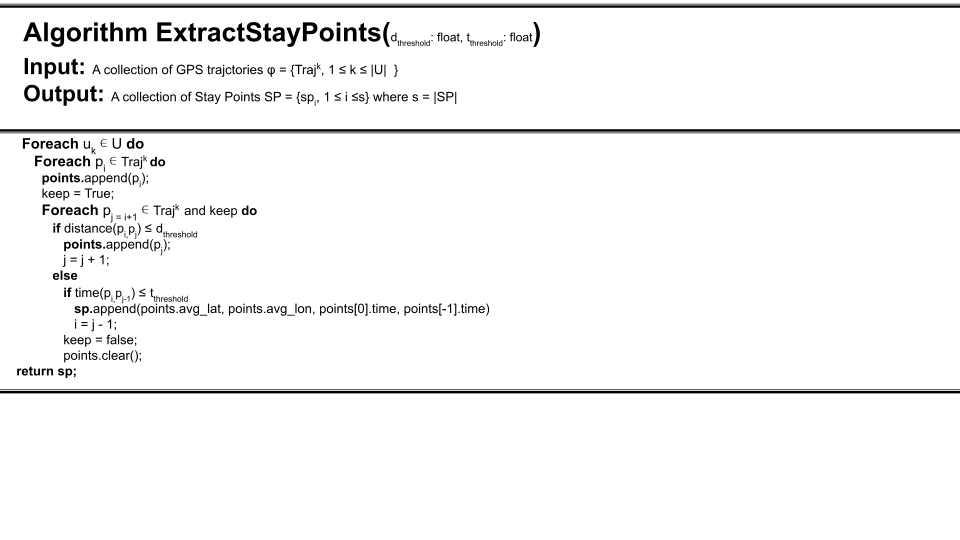
\includegraphics{images/sp.png}
    \caption{Stay point Extraction algorithm}\label{fig:extraction_sp}
\end{figure}

\paragraph{Cluster}
From the staypoint extracted we generated the clusters by using DBscan and as eps (maximum distance between two points to be considered neighbor) 
300 meters because we think that a stay point should work in a radius of 300 meters. Then we used the centroid of each cluster to ask Place APIs, from Google, 
which categories of business activty were found, we save the nearest one and we use as time for that activity the 0.5 quantile of the time of arrival in UTC format for each sp in the cluster.
We had to cluster the stay points because Place API is not free and the sp we found were really a lot. Probably with a free API we could train a more precise model.

\paragraph{Human activity}
Because we can't know which activity were doing the users in that SP, since it is created from a lot of sp of the users, we generated it randomly 
because an average of all was less meaning. We thought that a restaurant should be recommended when the user is walking or is still, because
the most frequently situation when a user need to find some place to eat is when he do some walking activity, like visiting the city center.
Instead for sport or leisure we generated also activity as car, bus or bike besides walk and still. The main thought was that when a user is moving with 
some transport he is going to hang out and want to have fun or maybe is going in same green space to take a walk or run.
We also converted the time, from each TZ, in UTC format to a time per day, i. e. instead of counting the time sine 01/01/1970 we converted the date in seconds starting from midnight and 
in day of week. Without these every date would be different and no meaning could be extracted.

\paragraph{Model}
After the synthetization of the dataset we trained a model based on a decision tree and used pickle to dump the weight into a .sav file so the model can be loaded 
every time is needed. This is used also when retrain a model with user's feedback.
\\
By doing this we generated a dataset with clustered stay point were we can infer, thanks to a Decision Tree, which place should be recommended by 
receiving as input the user position, his human activity and the actual time.

\end{document}